%%%%%%%%%%%%%%%%%%%%%%%%%%%%%%%%%%%%%%%%%
% Arsclassica Article
% LaTeX Template
% Version 1.1 (10/6/14)
%
% This template has been downloaded from:
% http://www.LaTeXTemplates.com
%
% Original author:
% Lorenzo Pantieri (http://www.lorenzopantieri.net) with extensive modifications by:
% Vel (vel@latextemplates.com)
%
% License:
% CC BY-NC-SA 3.0 (http://creativecommons.org/licenses/by-nc-sa/3.0/)
%
%%%%%%%%%%%%%%%%%%%%%%%%%%%%%%%%%%%%%%%%%

%----------------------------------------------------------------------------------------
%	PACKAGES AND OTHER DOCUMENT CONFIGURATIONS
%----------------------------------------------------------------------------------------

\documentclass[
10pt, % Main document font size
a4paper, % Paper type, use 'letterpaper' for US Letter paper
oneside, % One page layout (no page indentation)
%twoside, % Two page layout (page indentation for binding and different headers)
headinclude,footinclude, % Extra spacing for the header and footer
BCOR5mm, % Binding correction
]{scrartcl}

%%%%%%%%%%%%%%%%%%%%%%%%%%%%%%%%%%%%%%%%%
% Arsclassica Article
% Structure Specification File
%
% This file has been downloaded from:
% http://www.LaTeXTemplates.com
%
% Original author:
% Lorenzo Pantieri (http://www.lorenzopantieri.net) with extensive modifications by:
% Vel (vel@latextemplates.com)
%
% License:
% CC BY-NC-SA 3.0 (http://creativecommons.org/licenses/by-nc-sa/3.0/)
%
%%%%%%%%%%%%%%%%%%%%%%%%%%%%%%%%%%%%%%%%%

%----------------------------------------------------------------------------------------
%	REQUIRED PACKAGES
%----------------------------------------------------------------------------------------

\usepackage[
nochapters, % Turn off chapters since this is an article        
beramono, % Use the Bera Mono font for monospaced text (\texttt)
eulermath,% Use the Euler font for mathematics
pdfspacing, % Makes use of pdftex’ letter spacing capabilities via the microtype package
dottedtoc % Dotted lines leading to the page numbers in the table of contents
]{classicthesis} % The layout is based on the Classic Thesis style

\usepackage{arsclassica} % Modifies the Classic Thesis package

\usepackage[T1]{fontenc} % Use 8-bit encoding that has 256 glyphs

\usepackage[utf8]{inputenc} % Required for including letters with accents

\usepackage{graphicx} % Required for including images
\graphicspath{{Figures/}} % Set the default folder for images

\usepackage{enumitem} % Required for manipulating the whitespace between and within lists

\usepackage{lipsum} % Used for inserting dummy 'Lorem ipsum' text into the template

\usepackage{subfig} % Required for creating figures with multiple parts (subfigures)

\usepackage{amsmath,amssymb,amsthm} % For including math equations, theorems, symbols, etc

\usepackage{varioref} % More descriptive referencing

%----------------------------------------------------------------------------------------
%	THEOREM STYLES
%---------------------------------------------------------------------------------------

\theoremstyle{definition} % Define theorem styles here based on the definition style (used for definitions and examples)
\newtheorem{definition}{Definition}

\theoremstyle{plain} % Define theorem styles here based on the plain style (used for theorems, lemmas, propositions)
\newtheorem{theorem}{Theorem}

\theoremstyle{remark} % Define theorem styles here based on the remark style (used for remarks and notes)

%----------------------------------------------------------------------------------------
%	HYPERLINKS
%---------------------------------------------------------------------------------------

\hypersetup{
%draft, % Uncomment to remove all links (useful for printing in black and white)
colorlinks=true, breaklinks=true, bookmarks=true,bookmarksnumbered,
urlcolor=webbrown, linkcolor=RoyalBlue, citecolor=webgreen, % Link colors
pdftitle={}, % PDF title
pdfauthor={\textcopyright}, % PDF Author
pdfsubject={}, % PDF Subject
pdfkeywords={}, % PDF Keywords
pdfcreator={pdfLaTeX}, % PDF Creator
pdfproducer={LaTeX with hyperref and ClassicThesis} % PDF producer
} % Include the structure.tex file which specified the document structure and layout

\usepackage{appendix}
% \usepackage{float}
% \usepackage{subfig}
\usepackage{caption}
\usepackage{subcaption}   % handles objects not covered by caption

\hyphenation{Fortran hy-phen-ation} % Specify custom hyphenation points in words with dashes where you would like hyphenation to occur, or alternatively, don't put any dashes in a word to stop hyphenation altogether

%----------------------------------------------------------------------------------------
%	TITLE AND AUTHOR(S)
%----------------------------------------------------------------------------------------

\title{\normalfont\spacedallcaps{BioMap}} % The article title

\subtitle{\normalfont\spacedlowsmallcaps{Prototype Report}}

\author{\spacedlowsmallcaps{Graeme Faul\textsuperscript{1} \& Gregory Linklater\textsuperscript{1}}} % The article author(s) - author affiliations need to be specified in the AUTHOR AFFILIATIONS block

\date{\today} % An optional date to appear under the author(s)

%----------------------------------------------------------------------------------------

\begin{document}

%----------------------------------------------------------------------------------------
%	HEADERS
%----------------------------------------------------------------------------------------

\renewcommand{\sectionmark}[1]{\markright{\spacedlowsmallcaps{#1}}} % The header for all pages (oneside) or for even pages (twoside)
%\renewcommand{\subsectionmark}[1]{\markright{\thesubsection~#1}} % Uncomment when using the twoside option - this modifies the header on odd pages
\lehead{\mbox{\llap{\small\thepage\kern1em\color{halfgray} \vline}\color{halfgray}\hspace{0.5em}\rightmark\hfil}} % The header style

\pagestyle{scrheadings} % Enable the headers specified in this block

%----------------------------------------------------------------------------------------
%	TABLE OF CONTENTS & LISTS OF FIGURES AND TABLES
%----------------------------------------------------------------------------------------

\maketitle % Print the title/author/date block

\setcounter{tocdepth}{2} % Set the depth of the table of contents to show sections and subsections only

\tableofcontents % Print the table of contents

\listoffigures % Print the list of figures

% \listoftables % Print the list of tables

%----------------------------------------------------------------------------------------
%	AUTHOR AFFILIATIONS
%----------------------------------------------------------------------------------------

{\let\thefootnote\relax\footnotetext{\textsuperscript{1} \textit{Department of Computer Science, Rhodes University, Grahamstown, South Africa}}}

%----------------------------------------------------------------------------------------

\newpage % Start the article content on the second page, remove this if you have a longer abstract that goes onto the second page

%----------------------------------------------------------------------------------------
%	CONTENT
%----------------------------------------------------------------------------------------

\section{Introduction} % (fold)
\label{sec:introduction}



% section introduction (end)

\section{Application Description} % (fold)
\label{sec:application_description}

% section application_description (end)

\section{Prototype} % (fold)
\label{sec:prototype}

% section prototype (end)

\section{Conclusion} % (fold)
\label{sec:conclusion}

% section conclusion (end)

\newpage

%----------------------------------------------------------------------------------------
%	BIBLIOGRAPHY
%----------------------------------------------------------------------------------------

% \renewcommand{\refname}{\spacedlowsmallcaps{References}} % For modifying the bibliography heading

% \bibliographystyle{apalike}

% \bibliography{sample.bib} % The file containing the bibliography

% \newpage

%----------------------------------------------------------------------------------------
% APPENDICES
%----------------------------------------------------------------------------------------

\begin{appendices}

\section{Wireframes} % (fold)
\label{sec:wireframes}

\subsection{Login} % (fold)
\label{sub:login}

\begin{figure}[htb]
\centering 
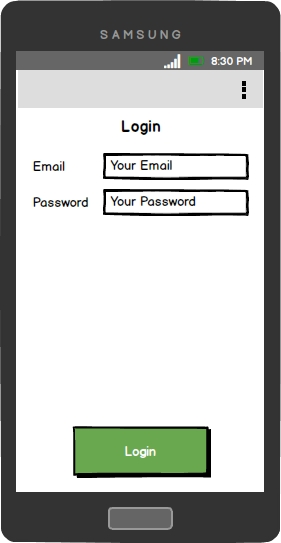
\includegraphics[width=.35\columnwidth]{LoginScreen} 
\caption{Login Screen Wireframe} % The text in the square bracket is the caption for the list of figures while the text in the curly brackets is the figure caption
\label{wire:login} 
\end{figure}

% subsection login (end)

\subsection{Home} % (fold)
\label{sub:home}

\begin{figure}[htb]
\centering 
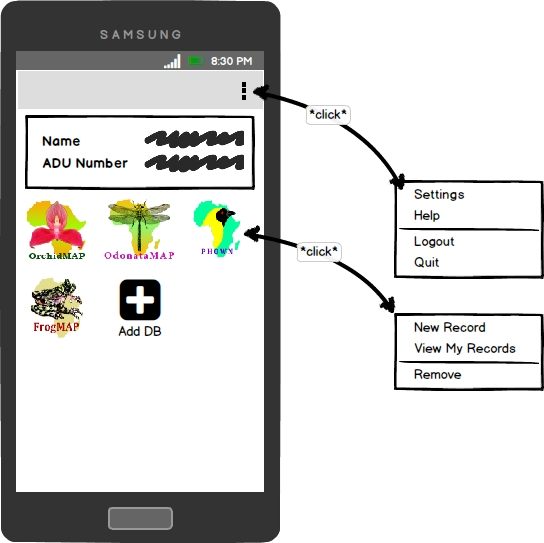
\includegraphics[width=.65\columnwidth]{HomeScreen} 
\caption{Home Screen Wireframe}
\label{wire:home} 
\end{figure}

\begin{figure}[htb]
\centering 
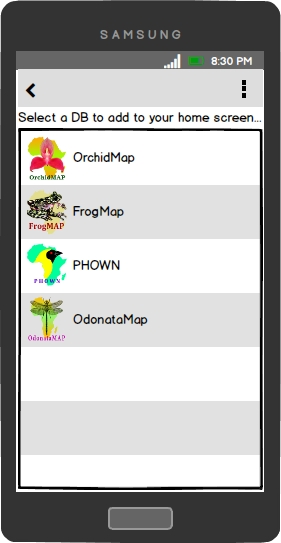
\includegraphics[width=.35\columnwidth]{AddDBScreen} 
\caption{Add Database Shortcut Screen Wireframe} 
\label{wire:add_db} 
\end{figure}

% subsection home (end)

\newpage

\subsection{Settings} % (fold)
\label{sub:settings}

\begin{figure}[htb]
\centering 
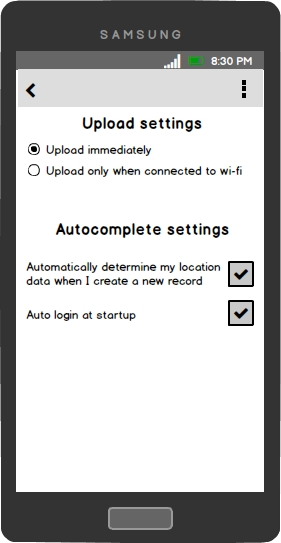
\includegraphics[width=.35\columnwidth]{SettingsScreen} 
\caption{Settings Screen Wireframe} 
\label{wire:settings} 
\end{figure}

% subsection settings (end)

\newpage

\subsection{Help} % (fold)
\label{sub:help}

\begin{figure}[h]
\centering
\begin{subfigure}{.5\columnwidth}
  \centering
  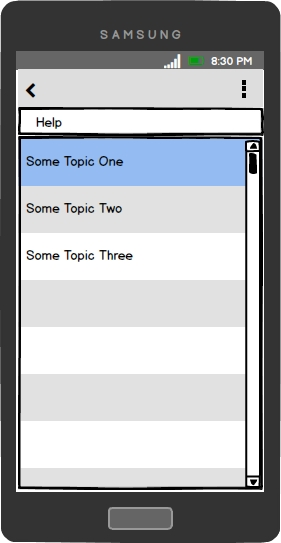
\includegraphics[width=.8\textwidth]{HelpHomeScreen}
  \caption{Select Help Topic Screen}
  \label{wire:help_home}
\end{subfigure}%
\begin{subfigure}{.5\columnwidth}
  \centering
  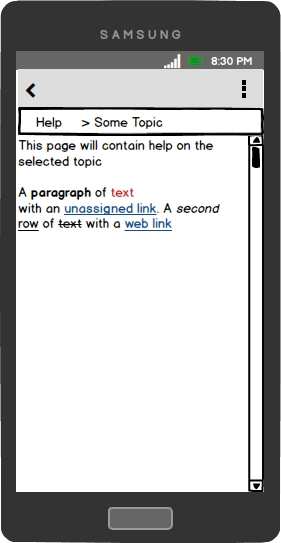
\includegraphics[width=.8\textwidth]{HelpTopicScreen}
  \caption{View Help Topic Screen}
  \label{wire:help_topic}
\end{subfigure}
\caption{User Help Wireframes}
\label{wire:help}
\end{figure}

% subsection help (end)

\newpage

\subsection{Record} % (fold)
\label{sub:record}

\begin{figure}[h]
\centering
\begin{subfigure}[b]{.475\textwidth}
  \centering
  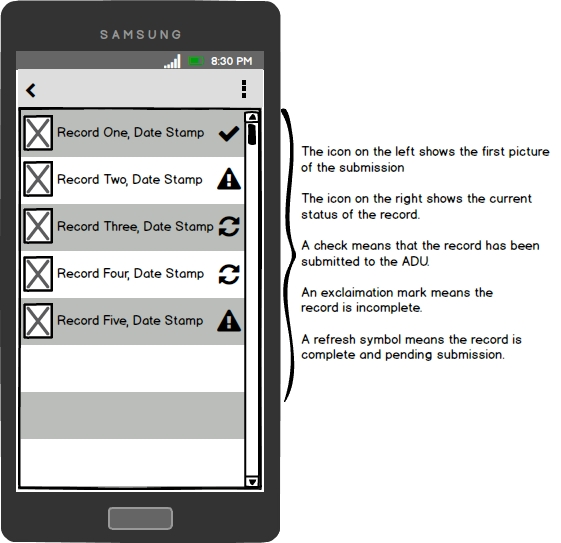
\includegraphics[width=.8\textwidth]{ViewRecordsScreen}
  \caption{Record List Screen Wireframe}
  \label{wire:records_list}
\end{subfigure}
\begin{subfigure}[b]{.475\textwidth}
  \centering
  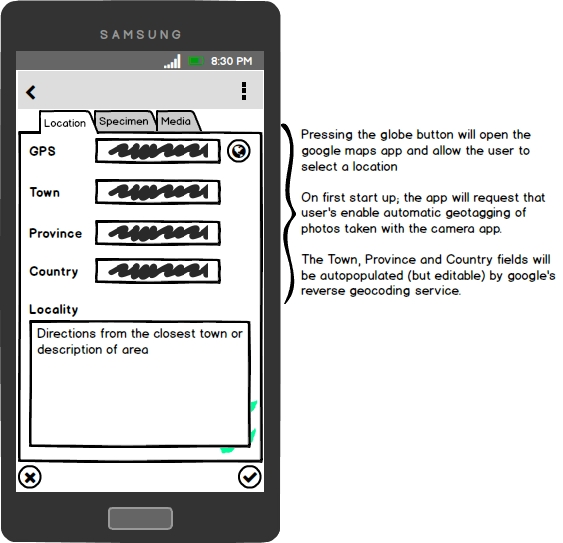
\includegraphics[width=.8\textwidth]{AddEditRecordLocation}
  \caption{Record Location Tab Wireframe}
  \label{wire:record_loc}
\end{subfigure}
\quad
\begin{subfigure}[b]{.475\textwidth}
  \centering
  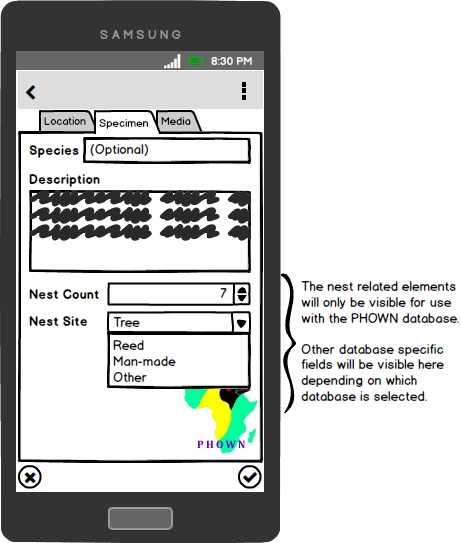
\includegraphics[width=.75\textwidth]{AddEditRecordSpecimen}
  \caption{Record Specimen Tab Wireframe}
  \label{wire:record_specimen}
\end{subfigure}
\begin{subfigure}[b]{.475\textwidth}
  \centering
  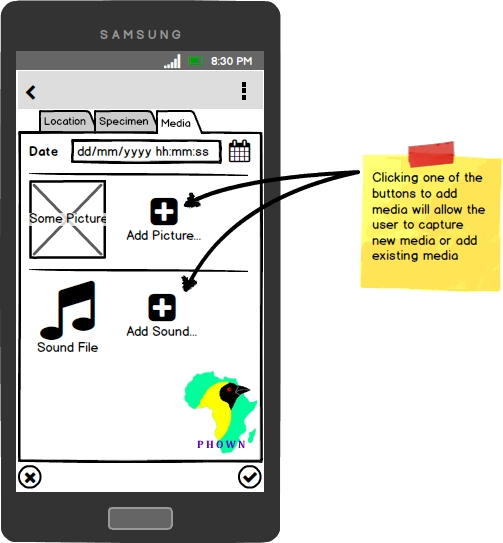
\includegraphics[width=.8\textwidth]{AddEditRecordMedia}
  \caption{Record Media Tab Wireframe}
  \label{wire:record_media}
\end{subfigure}
\caption{Record List and Detail Wireframes}
\label{wire:help}
\end{figure}

% subsection record (end)

% section wireframes (end)

\end{appendices}

\end{document}